% ==========================================================
% =                         ANEXOS                         =
% ==========================================================
%\phantomsection
\section{OLDatasets} \label{appendix:OLDatasets}

Standing for OpenLABEL Datasets, OLDatasets is a custom parser to convert any Dataset format to OpenLABEL format in order to integrate it with the \aclink{VCD} library ecosystem. Despite OLDatasets has been implemented as a custom Python module and it provides tools for developing parsers from any dataset into OpenLABEL for creating \aclink{BEV} reprojections of them, the parser currently only supports parsers for the NuImages dataset. Thus, the module currently provides three main features: common functionalities, which can be used for developing any dataset's parser; \aclink{BEV} functionalities, making use of the \aclink{BEV} reprojection module described in Section~\ref{sec:bev_reprojection_module}; and the NuImages parser.

The generation of the BEVDataset from the NuImages dataset takes the data structure shown in Figure~\ref{fig:nuimages_scheme} as input. This parser loops for each \texttt{sample\_data} of the NuImages dataset taking the front-camera images alongside the camera parametes and semantic annotations, resulting in the semantic class distribution defined in Table~\ref{tab:semantic_labels}.

\begin{figure}[!ht]
    \centering
    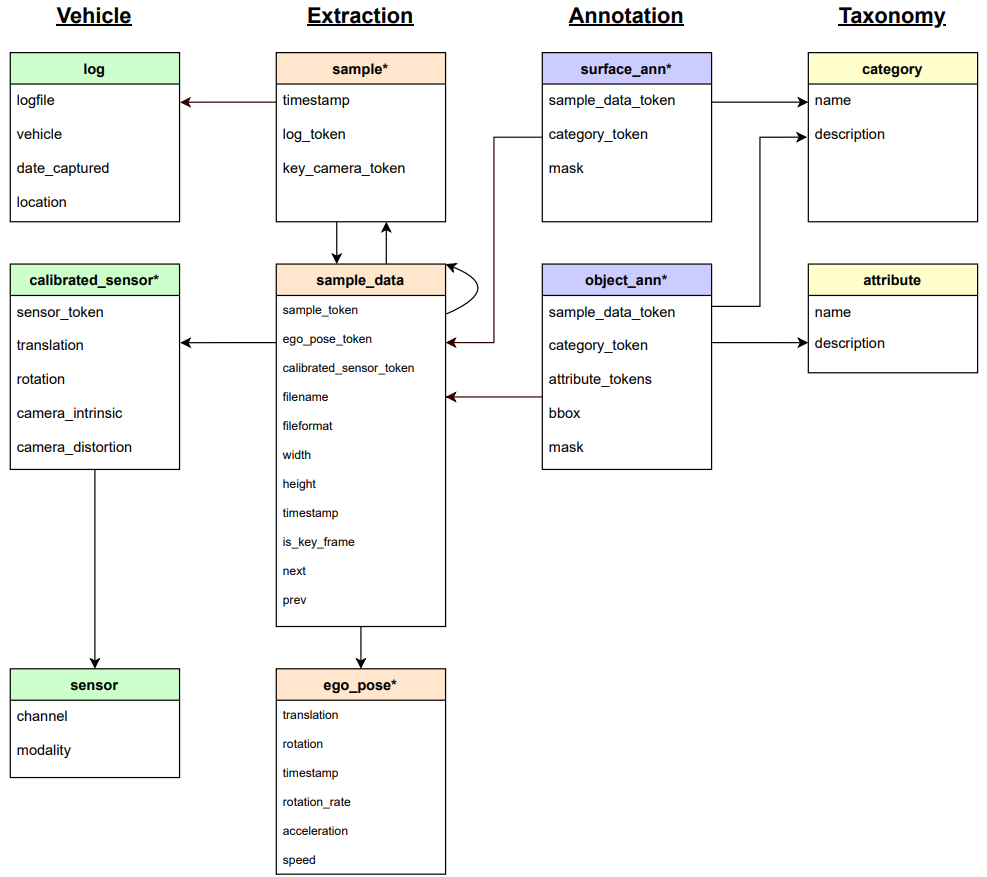
\includegraphics[width=0.6\linewidth]{images/appendix/NuImages_scheme.png}
    \caption{NuImages metadata scheme}
    \label{fig:nuimages_scheme}
\end{figure}
\begin{table}[!ht]
    \centering
    \tiny
    \begin{tabular}{l c c c c}
        \toprule
        \textbf{Name} & \textbf{ID} & \textbf{trainId} & \textbf{Dynamic} & \textbf{Color (RGB)} \\
        \midrule
        background                          & 0  & 0  & False & (0, 0, 0) \\
        animal                              & 1  & 1  & True  & (255, 0, 0) \\
        human.pedestrian.adult              & 2  & 2  & True  & (220, 20, 60) \\
        human.pedestrian.child              & 3  & 3  & True  & (220, 20, 60) \\
        human.pedestrian.construction\_worker & 4  & 4  & True  & (220, 20, 60) \\
        human.pedestrian.personal\_mobility & 5  & 5  & True  & (220, 20, 60) \\
        human.pedestrian.police\_officer    & 6  & 6  & True  & (220, 20, 60) \\
        human.pedestrian.stroller           & 7  & 7  & True  & (220, 20, 60) \\
        human.pedestrian.wheelchair         & 8  & 8  & True  & (220, 20, 60) \\
        movable\_object.barrier             & 9  & 9  & False & (190, 153, 153) \\
        movable\_object.debris              & 10 & 10 & False & (152, 251, 152) \\
        movable\_object.pushable\_pullable  & 11 & 11 & False & (255, 0, 0) \\
        movable\_object.trafficcone         & 12 & 12 & True  & (111, 74, 0) \\
        static\_object.bicycle\_rack        & 13 & 13 & False & (255, 0, 0) \\
        vehicle.bicycle                     & 14 & 14 & True  & (119, 11, 32) \\
        vehicle.bus.bendy                   & 15 & 15 & True  & (0, 60, 100) \\
        vehicle.bus.rigid                   & 16 & 16 & True  & (0, 60, 100) \\
        vehicle.car                         & 17 & 17 & True  & (0, 0, 142) \\
        vehicle.construction                & 18 & 18 & True  & (255, 0, 0) \\
        vehicle.emergency.ambulance         & 19 & 19 & True  & (255, 0, 0) \\
        vehicle.emergency.police            & 20 & 20 & True  & (255, 0, 0) \\
        vehicle.motorcycle                  & 21 & 21 & True  & (0, 0, 230) \\
        vehicle.trailer                     & 22 & 22 & True  & (0, 0, 110) \\
        vehicle.truck                       & 23 & 23 & True  & (0, 0, 70) \\
        vehicle.ego                         & 24 & 24 & True  & (255, 255, 255) \\
        flat.driveable\_surface             & 25 & 25 & False & (128, 64, 128) \\
        \midrule
        ignore                              & 255 & 255 &       &        \\
        \bottomrule
    \end{tabular}
    \caption{Semantic labels defined for NuImages masks}
    \label{tab:semantic_labels}
\end{table}

Once the BEVDataset is generated it is splitted into the "train", "val" and "test" sets using the postprocesing package of OLDatasets. The final class distribution of the BEVDataset is shown in Figure~\ref{fig:dataset_class_balance_combined}, where the absolute and relative pixel distribution per class is presented for perspective and \aclink{BEV} images. 

\begin{figure}[!ht]
    \centering
    \begin{subfigure}[b]{0.48\textwidth}
        \centering
        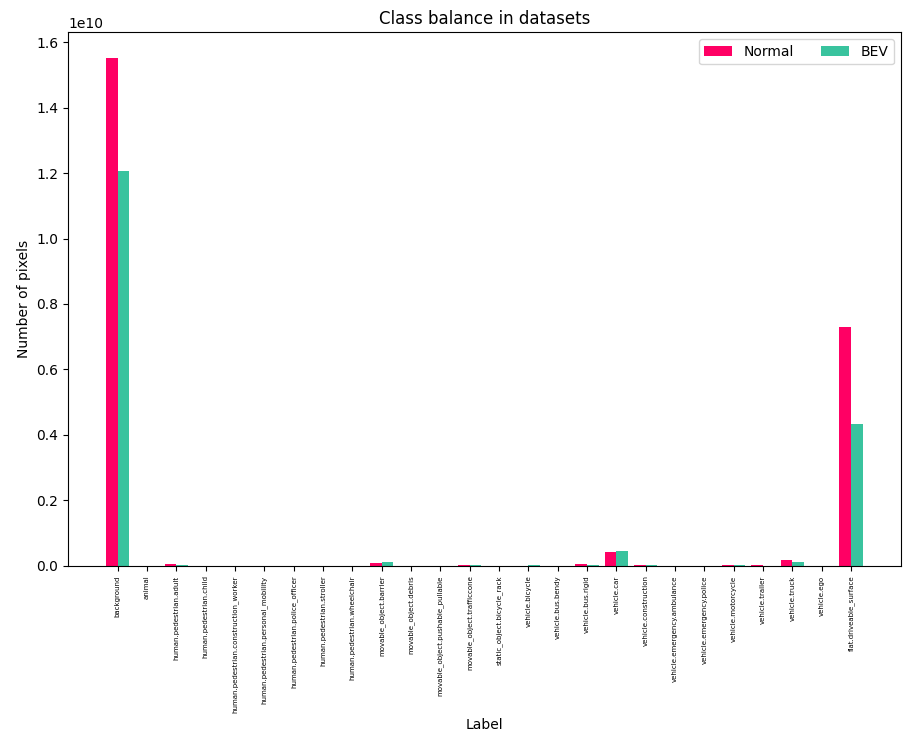
\includegraphics[width=\linewidth]{images/appendix/dataset_class_balance_pixels.png}
        \caption{Number of pixels per class}
        \label{fig:dataset_class_balance_pixels}
    \end{subfigure}
    \hfill
    \begin{subfigure}[b]{0.48\textwidth}
        \centering
        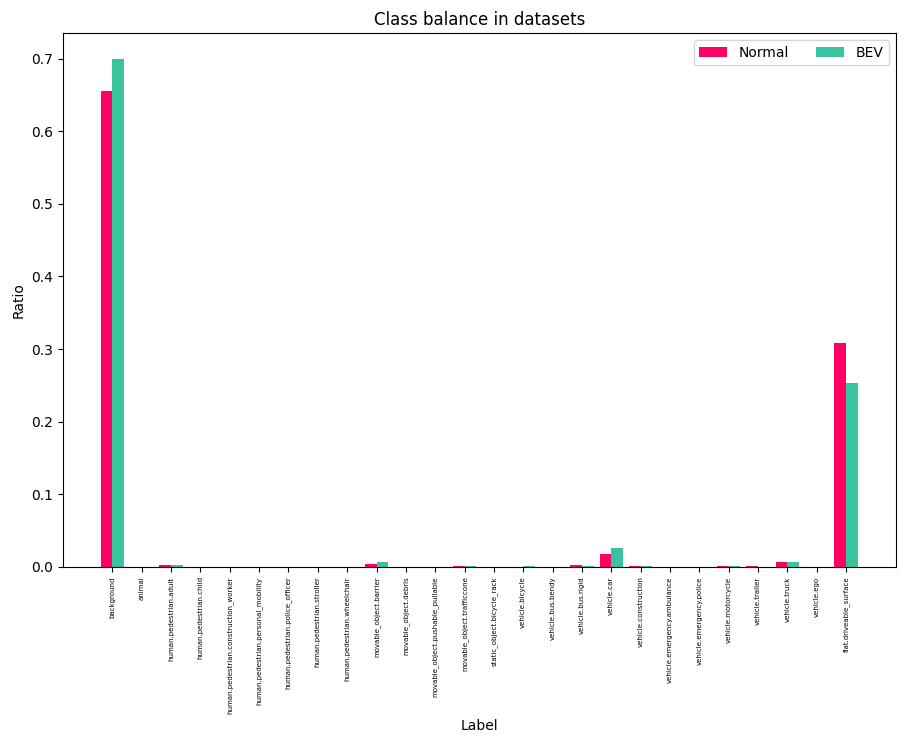
\includegraphics[width=\linewidth]{images/appendix/dataset_class_balance_ratio.png}
        \caption{Relative distribution of classes}
        \label{fig:dataset_class_balance_ratio}
    \end{subfigure}
    \caption{Class Balance in Datasets: (a) Pixel count per class and (b) Relative class distribution.}
    \label{fig:dataset_class_balance_combined}
\end{figure}

\newpage
% ==========================================================


% ==========================================================
\section{F1-Score vs Intersection Over Union} \label{appendix:f1_iou}
The objective of this appendix is to prove that Intersection over Union (\aclink{IoU}) and F1-Score are positive correlated and that \aclink{IoU} represents the worst case scenenario performance while F1-Score represents the average performance.

\begin{equation}
    \begin{aligned}
    \text{F1} &= \frac{2TP}{2TP + FP + FN} \\
    \text{IoU} &= \frac{TP}{TP + FP + FN}
    \end{aligned}
\end{equation}
    
% Step 1: Solve F1 in terms of IoU
\noindent
We know that:
\[
\text{IoU} = \frac{TP}{TP + FP + FN} \Rightarrow TP + FP + FN = \frac{TP}{\text{IoU}}
\]

\begin{equation}
    \begin{aligned}
        \text{F1} &= \frac{2TP}{2TP + FP + FN} = \frac{2TP}{TP + (TP + FP + FN)} = \frac{2TP}{TP + \frac{TP}{\text{IoU}}} \\
        &= \frac{2TP}{TP \left(1 + \frac{1}{\text{IoU}}\right)} = \frac{2}{1 + \frac{1}{\text{IoU}}} = \frac{2\text{IoU}}{1 + \text{IoU}}
    \end{aligned}
\end{equation}
    

% Step 2: Solve IoU in terms of F1
\noindent
Now solve for \(\text{IoU}\) in terms of \(\text{F1}\):
\[
\text{F1} = \frac{2\text{IoU}}{1 + \text{IoU}}
\]
    
\[
\text{F1}(1 + \text{IoU}) = 2\text{IoU}
\Rightarrow \text{F1} + \text{F1} \cdot \text{IoU} = 2 \cdot \text{IoU}
\]
    
\[
\text{F1} = 2\text{IoU} - \text{F1} \cdot \text{IoU}
\Rightarrow \text{F1} = \text{IoU}(2 - \text{F1})
\]
    
\[
\text{IoU} = \frac{\text{F1}}{2 - \text{F1}}
\]
    
\begin{equation}
    \boxed{
    \text{F1} = \frac{2\text{IoU}}{1 + \text{IoU}} \qquad
    \text{IoU} = \frac{\text{F1}}{2 - \text{F1}}
    }
    \label{eq:conversion}
\end{equation}

\aclink{IoU} is generally considered a "worst-case scenario" metric because its denominator, representing the union of predicted and true areas, heavily penalizes any mismatch. This makes it very sensitive to precise boundary alignment. In contrast, F1-Score provides a more "average performance" view by balancing precision and recall. 

\newpage
% ==========================================================


% ==========================================================
\section{Annotation BEV masks generation} \label{appendix:bev_masks_generation}
\begin{algorithm}
    \caption{Occupancy, occlusion and driveable mask generation}
    \label{algorithm:occ_masks}
    \scriptsize

    \begin{algorithmic}[1]
        % Input-Output
        \State \textbf{Input:} Initial BEV semantic mask $\mathcal{M}^{BEV}_{\left[h \times w\right]}$, panoptic data with 3D instance detections  $\mathcal{D}_{panoptic}$ and the set of selected labels for computing the semantic masks $\mathcal{L}_{sel}$
        \State \textbf{Output:} Final composite BEV mask $\mathcal{M}^{final}_{\left[h \times w\right]}$
        
        % Initialization
        \State \textbf{Initialize:}
        \State $\mathcal{M}^{final}_{\left[h \times w\right]}, \mathcal{M}^{occupancy}_{\left[h \times w\right]}, \mathcal{M}^{occlusion}_{\left[h \times w\right]} \gets \mathbf{0}$
        \State $\text{IntersectionFactors} \gets \text{empty dictionary}$ \Comment{Initialize structure to store intersection factors}
        
        % Main
        \State \textbf{Main:}        
        \For{each $\mathcal{I}_{sem}$ in $\mathcal{D}_{panoptic}$}
            \If{$\mathcal{I}_{sem}[\text{'dynamic'}]$ is \textbf{False} or $\mathcal{I}_{sem}[\text{'label'}] \notin \mathcal{L}_{sel}$}
                \State \textbf{continue}
                \Comment{Skip if it is not dynamic or has not been selected.}
            \EndIf
        
            \State $M_{ccomps} \gets \text{connectedComponents}(\mathcal{M}^{BEV}_{\left[h \times w\right]} == \mathcal{I}_{sem}[\text{'label\_id'}])$



            % Compute intersection factors:
            \For{each $B_{3D}$ in $\mathcal{I}_{sem}[\text{'instance\_3dboxes'}]$} \Comment{Compute intersection factors}
                \State $\text{Factors}_{B_{3D}} \gets \text{empty list}$
                \State $B_{mask} \gets \text{create\_binary\_mask\_of\_cuboid\_base}(B_{3D}, h, w)$
                
                \State $\mathcal{M}^{occupancy}_{\left[h \times w\right]} \lor = B_{mask}$

                \For{each $M_{c}$ in $M_{ccomps}$}
                    \State $\text{Factors}_{B_{3D}}.\text{append}(\text{compute\_IoU}(M_{c}, B_{mask}))$
                \EndFor
                \State $\text{IntersectionFactors}[B_{3D}] \gets \text{Factors}_{B_{3D}}$
            \EndFor


            % Assign connected components to cuboids and draw them in the M_occupancy and M_occlusion
            \For{$j \gets 0 \text{ to } \text{len}(M_{ccomps})$} \Comment{Assign connected components to cuboids}
                \State $\text{max\_val} \gets 0$
                \State $\text{best\_bbox\_id} \gets -1$
                \For{$i \gets 0 \text{ to } \text{len}(\mathcal{I}_{sem}[\text{'instance\_3dboxes'}])-1$}
                    \State $B_{inst\_id} \gets \mathcal{I}_{sem}[\text{'instance\_3dboxes'}][i][\text{'inst\_id'}]$
                    \State $f \gets \text{IntersectionFactors}[B_{inst\_id}][j]$
                    \If{$f > \text{max\_val}$}
                        \State $\text{max\_val} \gets f$
                        \State $\text{best\_bbox\_id} \gets B_{inst\_id}$
                    \EndIf
                \EndFor

                \If{$\text{max\_val} > 0$}
                    \State $\mathcal{M}^{occlusion}_{\left[h \times w\right]} \lor = M_{ccomps}[j]$
                \EndIf
            \EndFor

        \EndFor
        
        % Combine all masks into final output
        \State $\mathcal{M}^{final}_{\left[h \times w\right]}[\mathcal{M}^{BEV}_{\left[h \times w\right]}[\text{'driveable'}]] \gets \text{label\_driveable\_id}$
        \Comment{Assign drivable area}
        \State $\mathcal{M}^{final}_{\left[h \times w\right]}[\mathcal{M}^{occlusion}_{\left[h \times w\right]} == 1] \gets \text{label\_occluded\_id}$
        \Comment{Assign occluded area}
        \State $\mathcal{M}^{final}_{\left[h \times w\right]}[\mathcal{M}^{occupancy}_{\left[h \times w\right]} == 1] \gets \text{label\_occuped\_id}$
        \Comment{Assign occuped area}
        
        % Return
        \State \Return $\mathcal{M}^{final}_{\left[h \times w\right]}$
    \end{algorithmic}
\end{algorithm}
\newpage
% ==========================================================


% ==========================================================
\section{Trained model's hyperparameters} \label{appendix:models_hyperparameters}
For clarity and to maintain the flow of discussion, the primary text of this thesis refers to models conceptually rather than by their specific internal names. This section, however, establishes the mapping between the experimental results presented in the multiple experimental sections and their corresponding model configurations listed in Table~\ref{tab:models_hyperparameters}, ensuring full reproducibility.

The models that follow the \textit{Segmenting-Then-IPM} pipeline to obtain BEV semantic masks are referred to as \texttt{raw2segbev}, while those that first apply IPM and then perform segmentation are named \texttt{raw2bevseg}.

The initial training configurations for both the \textit{Segmenting-Then-IPM} and \textit{IPM-Then-Segmenting} strategies, discussed in Section~\ref{sec:bev2seg_2_experimentation} where models exhibit overfitting, correspond to models \texttt{raw2segbev\_mit-b0\_v0.2} and \texttt{raw2bevseg\_mit-b0\_v0.3}. Subsequently, model \texttt{raw2segbev\_mit-b0\_v0.2} is employed for the semantic merging comparison detailed in Section~\ref{sec:merging_labels}. In this comparison, model \texttt{raw2segbev\_mit-b0\_v0.4} incorporates the semantic merging strategy. The data augmentation techniques comparison, presented in Section~\ref{sec:data_augmentation}, employ the MiT-B0 models from Table~\ref{tab:models_hyperparameters} that implement the semantic merging strategy. Finally, Section~\ref{sec:bev2seg_2_comparison} encompasses all models with the exception of \texttt{raw2segbev\_mit-b0\_v0.2} and \texttt{raw2bevseg\_mit-b0\_v0.3}.

\begin{table}[!ht]
    \centering
    \begin{threeparttable} % Start threeparttable environment
        \tiny
        \begin{tabular}{l l | c c c c c c c c}
            \toprule
            \textbf{Model} & \textbf{MiT Type} & \textbf{Batch Size} & \textbf{Max Epochs} & \textbf{LR} & \textbf{WD} & \textbf{GA} & \textbf{ML} & \textbf{DA} & \textbf{CS} \\
            \midrule

            \multicolumn{10}{l}{\textbf{IPM Then Segmenting}} \\
            \midrule
            % Ejemplo de fila para un modelo
            raw2bevseg\_mit-b0\_v0.3 & MiT-B0 & 16 & 200 & 6e-5 & 0.0 & - & False & None & - \\
            
            raw2bevseg\_mit-b0\_v0.4 & MiT-B0 & 16 & 200 & 6e-5 & 0.0 & - & True & None & 14000 \\

            raw2bevseg\_mit-b0\_v0.5 & MiT-B0 & 16 & 200 & 6e-5 & 0.01 & - & True & Extrinsic & 40200 \\
            raw2bevseg\_mit-b0\_v0.6 & MiT-B0 & 16 & 200 & 6e-5 & 0.01 & - & True & Normal & 66000 \\
            

            raw2bevseg\_mit-b2\_v0.3 & MiT-B2 & 16 & 200 & 6e-5 & 0.01 & - & True & Extrinsic & 24800 \\
            raw2bevseg\_mit-b2\_v0.4 & MiT-B2 & 16 & 200 & 6e-5 & 0.01 & - & True & Normal & 26200 \\
            
            raw2bevseg\_mit-b4\_v0.1 & MiT-B4 & 8 & 200 & 6e-5 & 0.01 & 2 & True & Extrinsic & 16600 \\
            raw2bevseg\_mit-b4\_v0.2 & MiT-B4 & 8 & 200 & 6e-5 & 0.01 & 2 & True & Normal & 15800 \\
            
            \midrule[1pt]
            \multicolumn{10}{l}{\textbf{Segmenting Then IPM}} \\
            \midrule
            raw2segbev\_mit-b0\_v0.2 & MiT-B0 & 16 & 200 & 6e-5 & 0.0 & - & False & None & 11800 \\
            
            raw2segbev\_mit-b0\_v0.4 & MiT-B0 & 16 & 200 & 6e-5 & 0.0 & - & True & None & 9000 \\
            raw2segbev\_mit-b0\_v0.5 & MiT-B0 & 16 & 200 & 6e-5 & 0.01 & - & True & Normal & 7800 \\
            
            raw2segbev\_mit-b2\_v0.4 & MiT-B2 & 16 & 200 & 6e-5 & 0.01 & - & True & Normal & 40800 \\

            raw2segbev\_mit-b2\_v0.4 & MiT-B4 & 8 & 200 & 6e-5 & 0.01 & 2 & True & Normal & 20200 \\

            \bottomrule
        \end{tabular}
        \begin{tablenotes} % Table notes start here
            \item[] \textbf{LR}: Learning Rate; \textbf{WD}: Weight Decay; \textbf{GA}: Gradient Accumulation; \textbf{ML}: Merging Labels; \textbf{DA}: Data Augmentations; \textbf{CS}: Checkpoint Step.
        \end{tablenotes} % Table notes end here
    \end{threeparttable} % End threeparttable environment

    \caption{Used hyperparameters}
    \label{tab:models_hyperparameters}
\end{table}
\newpage
% ==========================================================


% ==========================================================
\section{Semantic merging with perspective masks}
This appendix presents an additional evaluation of the semantic merging comparison focusing on models \texttt{raw2segbev\_mit-b0\_v0.2} and \texttt{raw2segbev\_mit-b0\_v0.4}. Unlike the main discussion, this evaluation is performed using perspective semantic masks instead of BEV semantic masks. The results are summarized in Table~\ref{tab:merging_comparison_nor}. Despite the change in evaluation data, the conclusions remain consistent with those presented in Section~\ref{sec:merging_labels}.

\begin{table}[!ht]
    \centering
    \tiny
    \begin{tabular}{llcccc}
    \toprule
    \textbf{Merged Class} & \textbf{Original Label} & \textbf{mIoU A} & \textbf{mIoU B} & \textbf{mF1 A} & \textbf{mF1 B} \\
    \midrule
    background & background & 0.98 & 0.98 & 0.99 & 0.99 \\
    \midrule
    animal & animal & 0.00 & 0.00 & 0.00 & 0.00 \\
    \midrule
    human.pedestrian.adult & human.pedestrian.adult & 0.12 & 0.14 & 0.17 & 0.19 \\
     & human.pedestrian.child & 0.00 & - & 0.00 & - \\
     & human.pedestrian.construction\_worker & 0.01 & - & 0.01 & - \\
     & human.pedestrian.personal\_mobility & 0.00 & - & 0.00 & - \\
     & human.pedestrian.police\_officer & 0.00 & - & 0.00 & - \\
     & human.pedestrian.stroller & 0.00 & - & 0.00 & - \\
     & human.pedestrian.wheelchair & 0.00 & - & 0.00 & - \\
    \midrule
    movable\_object.barrier & movable\_object.barrier & 0.11 & 0.17 & 0.13 & 0.21 \\
     & movable\_object.debris & 0.00 & - & 0.00 & - \\
     & movable\_object.pushable\_pullable & 0.00 & - & 0.00 & - \\
     & movable\_object.trafficcone & 0.09 & - & 0.12 & - \\
     & static\_object.bicycle\_rack & 0.01 & - & 0.01 & - \\
    \midrule
    vehicle.car & vehicle.bus.bendy & 0.00 & - & 0.00 & - \\
     & vehicle.bus.rigid & 0.05 & - & 0.06 & - \\
     & vehicle.car & 0.48 & 0.58 & 0.56 & 0.66 \\
     & vehicle.construction & 0.02 & - & 0.03 & - \\
     & vehicle.emergency.ambulance & 0.00 & - & 0.00 & - \\
     & vehicle.emergency.police & 0.00 & - & 0.00 & - \\
     & vehicle.trailer & 0.00 & - & 0.00 & - \\
     & vehicle.truck & 0.14 & - & 0.16 & - \\
    \midrule
    vehicle.ego & vehicle.ego & 0.00 & 0.00 & 0.00 & 0.00 \\
    \midrule
    vehicle.motorcycle & vehicle.bicycle & 0.02 & - & 0.03 & - \\
     & vehicle.motorcycle & 0.06 & 0.07 & 0.07 & 0.09 \\
    \midrule
    flat.driveable\_surface & flat.driveable\_surface & 0.97 & 0.97 & 0.99 & 0.99 \\
    \bottomrule
     & & 0.12 & 0.36 & 0.13 & 0.39 \\
    \bottomrule
    \end{tabular}
    \caption{Per-class metric comparison between Model A and merged Model B evaluated with normal images}
    \label{tab:merging_comparison_nor}
\end{table}

\newpage
% ==========================================================


% ==========================================================
% \section{Color palette}
% \begin{table}[!ht]
%     \centering
%     \renewcommand{\arraystretch}{1.5} % Increase row height
%     \setlength{\tabcolsep}{12pt} % Increase column spacing
%     \begin{tabular}{c c}
%         \toprule
%         \textbf{Hex Code} & \textbf{Color Sample} \\
%         \midrule
%         \#FF0064 & \cellcolor[HTML]{FF0064} \hspace{2cm} \\
%         \#FF62A0 & \cellcolor[HTML]{FF62A0} \hspace{2cm} \\
%         \#0277BD & \cellcolor[HTML]{0277BD} \hspace{2cm} \\
%         \#2AB0D2 & \cellcolor[HTML]{2AB0D2} \hspace{2cm} \\
%         \#7700A0 & \cellcolor[HTML]{7700A0} \hspace{2cm} \\
%         \#B200EF & \cellcolor[HTML]{B200EF} \hspace{2cm} \\
%         \#00A032 & \cellcolor[HTML]{00A032} \hspace{2cm} \\
%         \#03FF52 & \cellcolor[HTML]{03FF52} \hspace{2cm} \\
%         \#FF9800 & \cellcolor[HTML]{FF9800} \hspace{2cm} \\
%         \#FFB03B & \cellcolor[HTML]{FFB03B} \hspace{2cm} \\
%         \#C00071 & \cellcolor[HTML]{C00071} \hspace{2cm} \\
%         \#FF37AD & \cellcolor[HTML]{FF37AD} \hspace{2cm} \\
%         \#00A697 & \cellcolor[HTML]{00A697} \hspace{2cm} \\
%         \#44FFEE & \cellcolor[HTML]{44FFEE} \hspace{2cm} \\
%         \bottomrule
%     \end{tabular}
%     \caption{Color Palette}
%     \label{tab:color_palette}
% \end{table}
